%% LyX 2.3.6 created this file.  For more info, see http://www.lyx.org/.
%% Do not edit unless you really know what you are doing.
\documentclass[english,aspectratio=169]{beamer}
\usepackage{lmodern}
\renewcommand{\sfdefault}{lmss}
\renewcommand{\ttdefault}{lmtt}
\usepackage[T1]{fontenc}
\usepackage[latin9]{inputenc}
\setlength{\parskip}{\medskipamount}
\setlength{\parindent}{0pt}
\usepackage{url}
\usepackage{amsbsy}
\usepackage{amssymb}
\usepackage{graphicx}
\PassOptionsToPackage{normalem}{ulem}
\usepackage{ulem}

\makeatletter

%%%%%%%%%%%%%%%%%%%%%%%%%%%%%% LyX specific LaTeX commands.
\pdfpageheight\paperheight
\pdfpagewidth\paperwidth


%%%%%%%%%%%%%%%%%%%%%%%%%%%%%% Textclass specific LaTeX commands.
% this default might be overridden by plain title style
\newcommand\makebeamertitle{\frame{\maketitle}}%
% (ERT) argument for the TOC
\AtBeginDocument{%
  \let\origtableofcontents=\tableofcontents
  \def\tableofcontents{\@ifnextchar[{\origtableofcontents}{\gobbletableofcontents}}
  \def\gobbletableofcontents#1{\origtableofcontents}
}

%%%%%%%%%%%%%%%%%%%%%%%%%%%%%% User specified LaTeX commands.
\usetheme{CambridgeUS}
\usecolortheme{dolphin}
\hypersetup{}
\usepackage{tikz}
\usepackage{color}
\usepackage{listings}


\makeatother

\usepackage{babel}
\usepackage{listings}
\renewcommand{\lstlistingname}{Listing}

\begin{document}
\title[M3-1]{Scalar and vector fields}
\author{Department of Oceanography}
\institute[UCT]{University of Cape Town}
\date{SEA3004F}
\makebeamertitle

\section*{Outlines}
\begin{frame}{Outline}

\tableofcontents{}
\end{frame}


\section{Scalar fields}
\begin{frame}{Scalars in ocean and atmosphere sciences}

\begin{itemize}
\item The typical scalars are temperature, pressure, humidity, irradiance,
precipitation, salinity, nutrient concentrations, abundances of organisms,
etc. \textbf{Scalars are usually considered constants, but in this
discipline this term is used for scalar fields.}
\item A \textbf{scalar field} is a multivariate function: $T(x,y,z,t)$
$\Rightarrow$ \textbf{multidimensional (N-dimensional, ND) array}
\item In 2D, it is a mapping representation of a matrix, in which each point
in the plane is associated to a value. The plane may be continuous
(the field is a mathematical function), or discrete (the field is
an array, which is the only way we have to visualize a field, e.g.
with octave)
\end{itemize}
\end{frame}
%
\begin{frame}[fragile]{Mathematical ``fields''}
\begin{columns}[t]

\column{8cm}

\begin{lstlisting}[language=Octave,basicstyle={\scriptsize},breaklines=true]
figure
peaks # this is the figure on the right
help peaks
# plot the peaks function using a different mesh
X = 0:0.1:2;
Y = -2:0.2:2;
[XX,YY]=meshgrid(X,Y);
figure
peaks(XX,YY)
xlabel('X')
ylabel('Y')
axis equal
# explore other ways to visualize the field in 2D and 3D
P = peaks(XX,YY);
figure # this is a 2D map (pseudocolor)
pcolor(XX,YY,P)
figure # this is a 3D line plot
plot3(XX,YY,P)
\end{lstlisting}


\column{6cm}

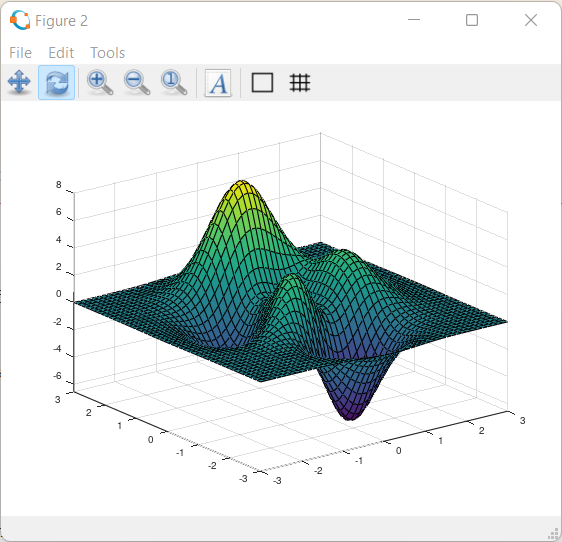
\includegraphics[width=5cm]{figures/M3/peaks}

Note that the field can be ``rotated'' by clicking on the highlighted
button in the menu
\end{columns}

\end{frame}
%
\begin{frame}[fragile]{An atmospheric ``mathematical'' field}

Consider the scalar field 
\[
\theta\left(x,y\right)=283+\frac{x^{2}+y^{2}}{15}
\]
with $x\in\left[-10,10\right]$ and $y\in\left[-10,10\right]$. Does
it look like an atmospheric feature?

\begin{lstlisting}[language=Octave,basicstyle={\scriptsize}]
x = -10:10; 
y = -10:10; 
help meshgrid % meshgrid is the function 
[X,Y] = meshgrid(x , y);
%Graph the scalar field 
figure 
T = 283+(X.^2+Y.^2)/15;
pcolor(X,Y,T)
colorbar
title('Air Temperature (K)')
print -dpng -r200 scalr_field_temperature.png
\end{lstlisting}

\end{frame}

\begin{frame}{Horizontal slicing of discrete scalar field (maps)}

\begin{columns}[t]


\column{9cm}

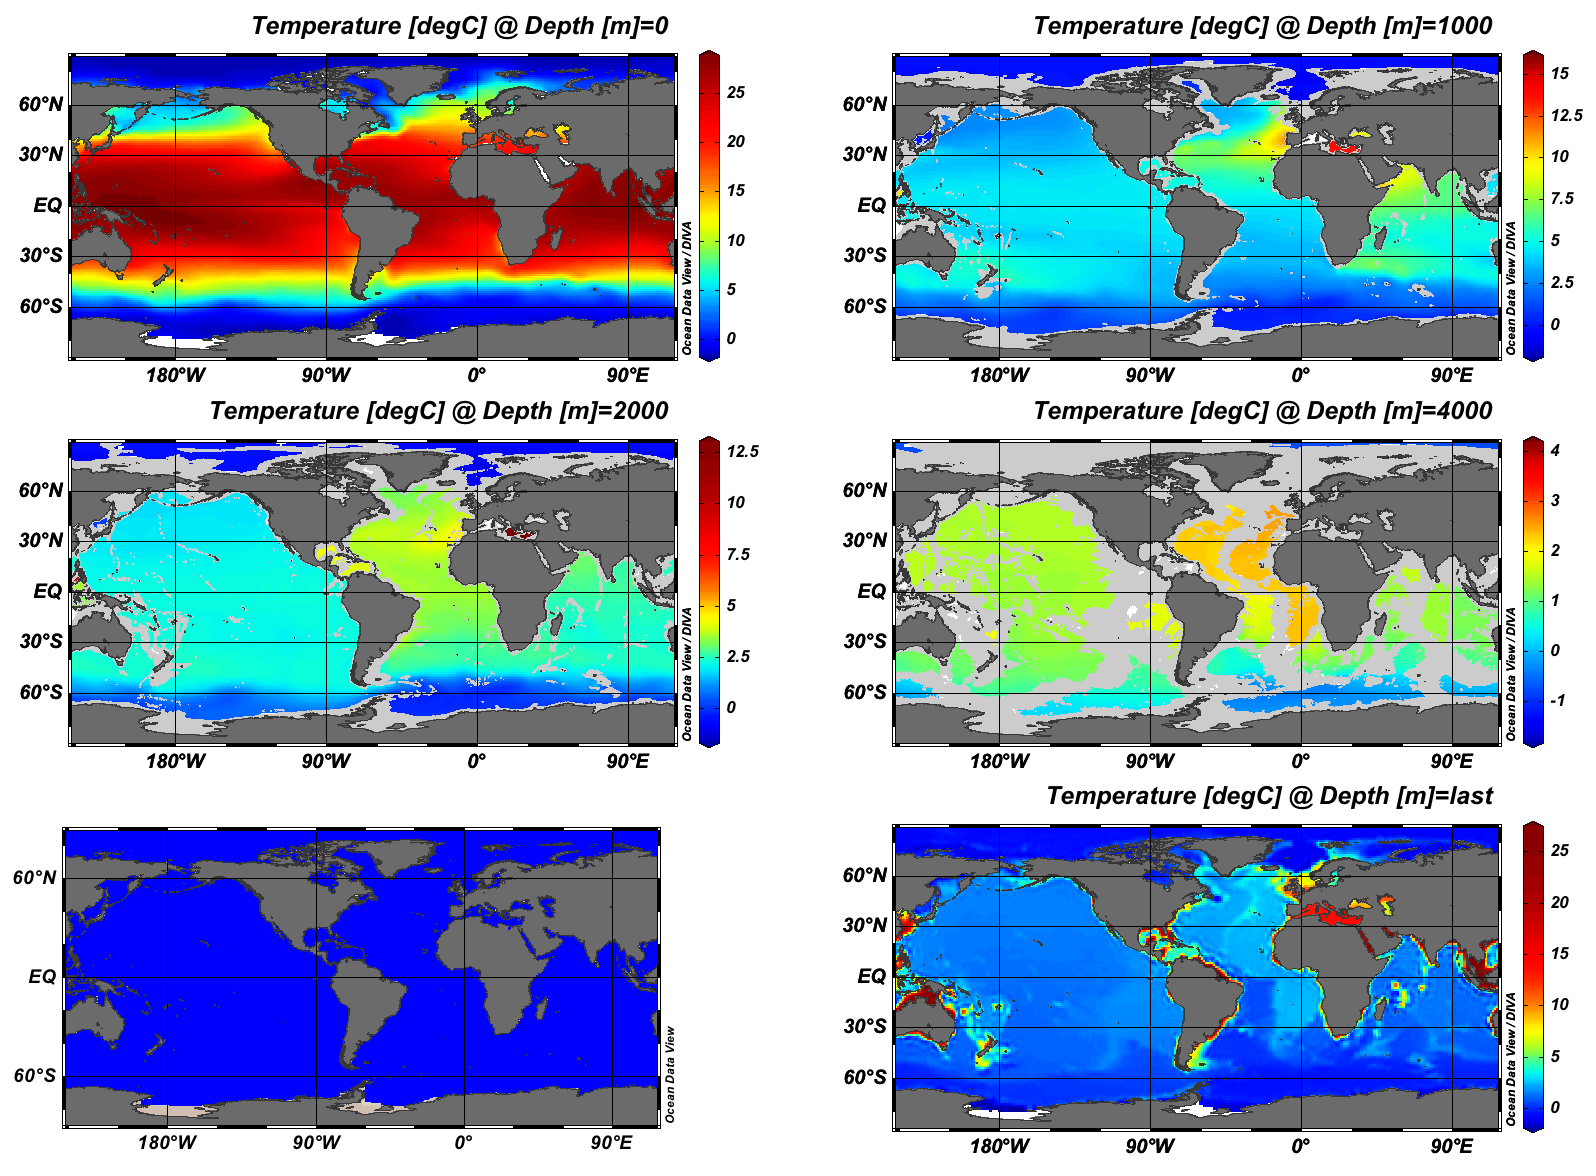
\includegraphics[width=9cm]{figures/M1/Temperature_maps_WOA13_ODV}

\column{3.5cm}
\begin{itemize}
\item {\small{}Temperature maps at various depth from the World Ocean Atlas
(WOA13) gridded dataset}{\small\par}
\item {\small{}The first 4 graphs are slices at given depths; the last one
is an iso-surface (bottom)}{\small\par}
\end{itemize}
\end{columns}

\end{frame}

\begin{frame}{Examples of scalar biogeochemical fields}

\begin{columns}[t]


\column{7cm}

\vspace{-0.5cm}
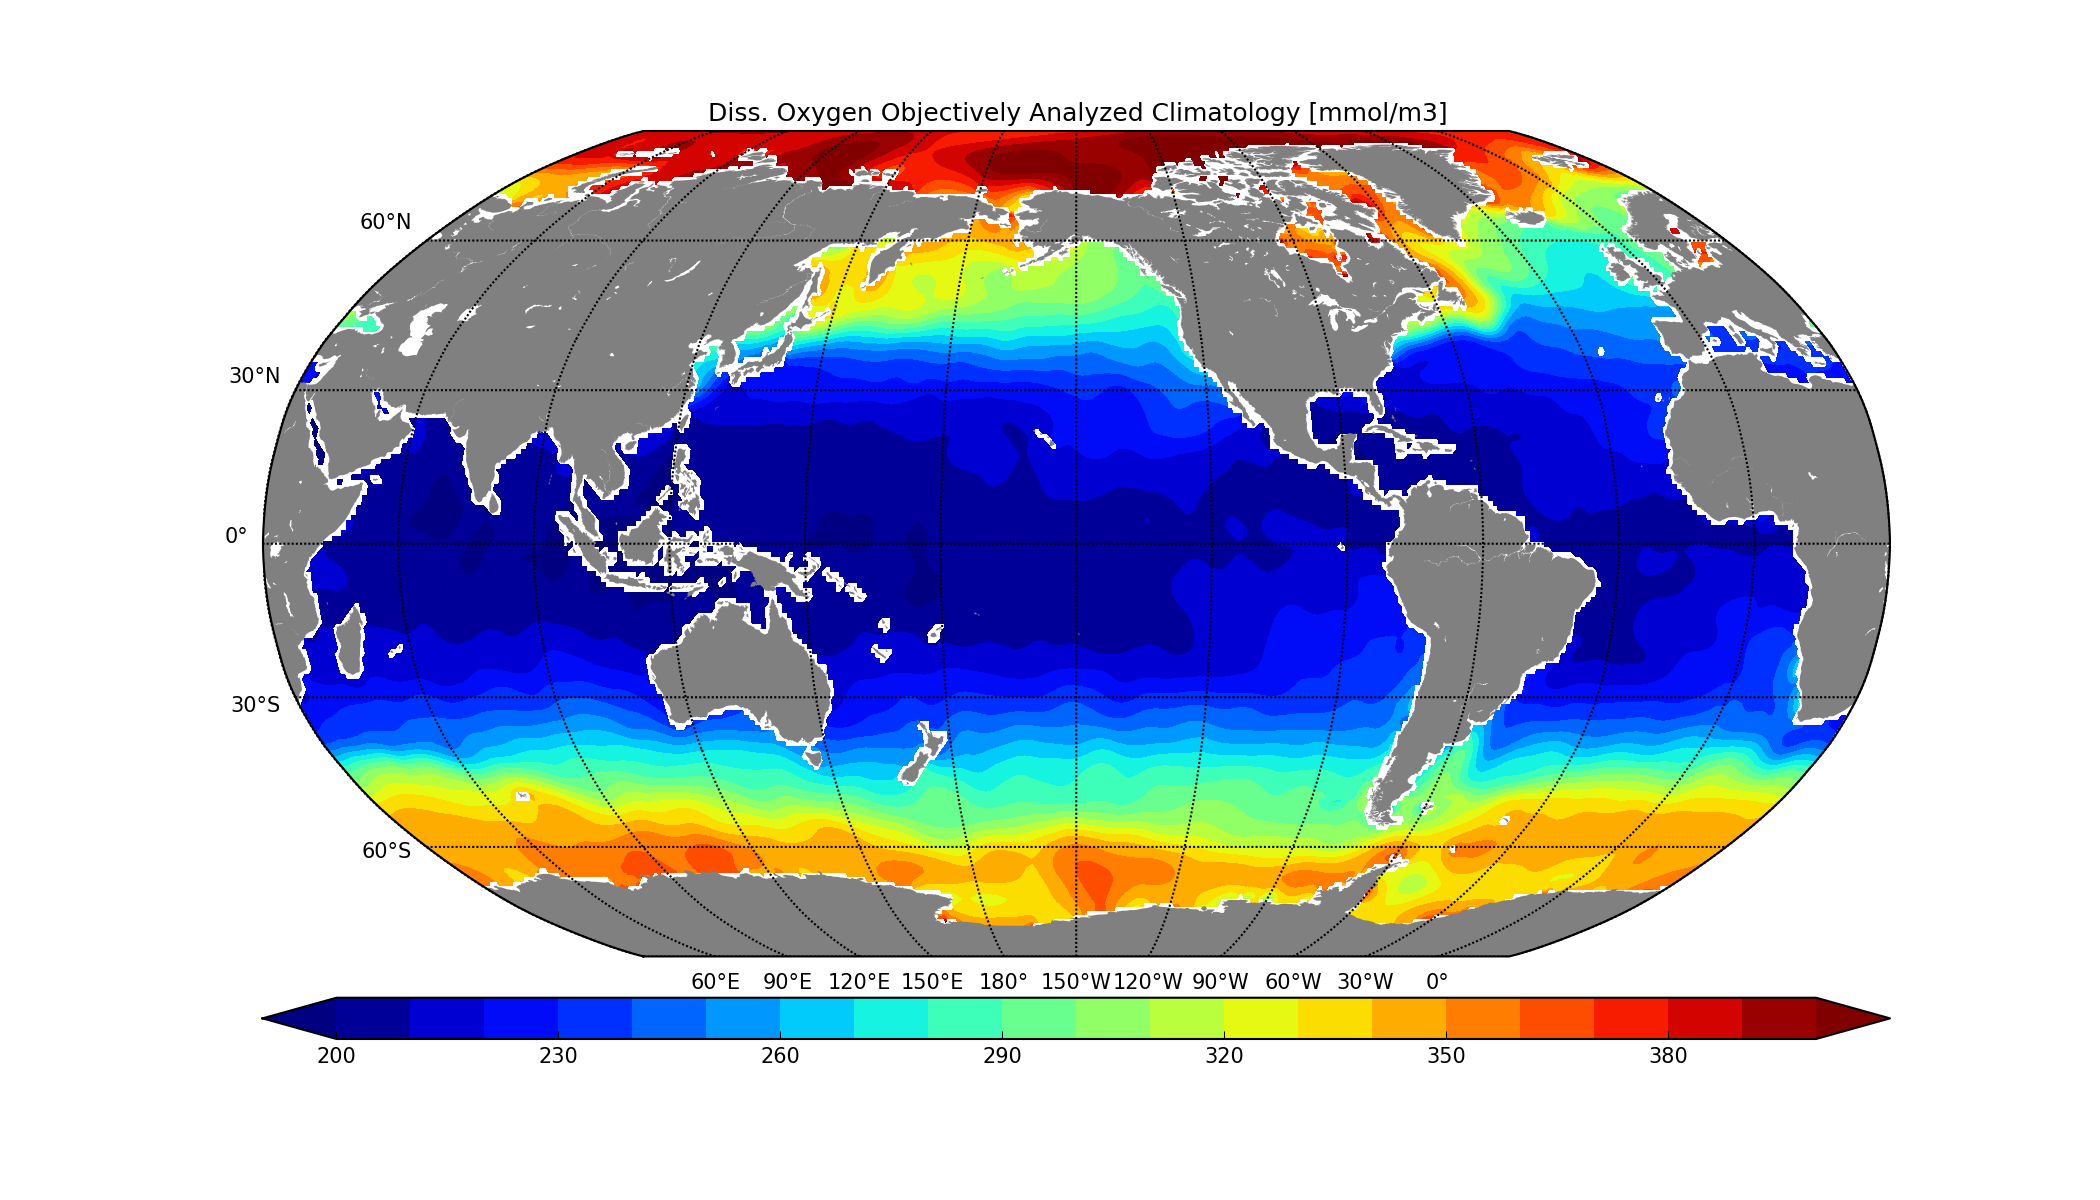
\includegraphics[width=7cm]{figures/M1/Oxygen_map_WOA9_python}

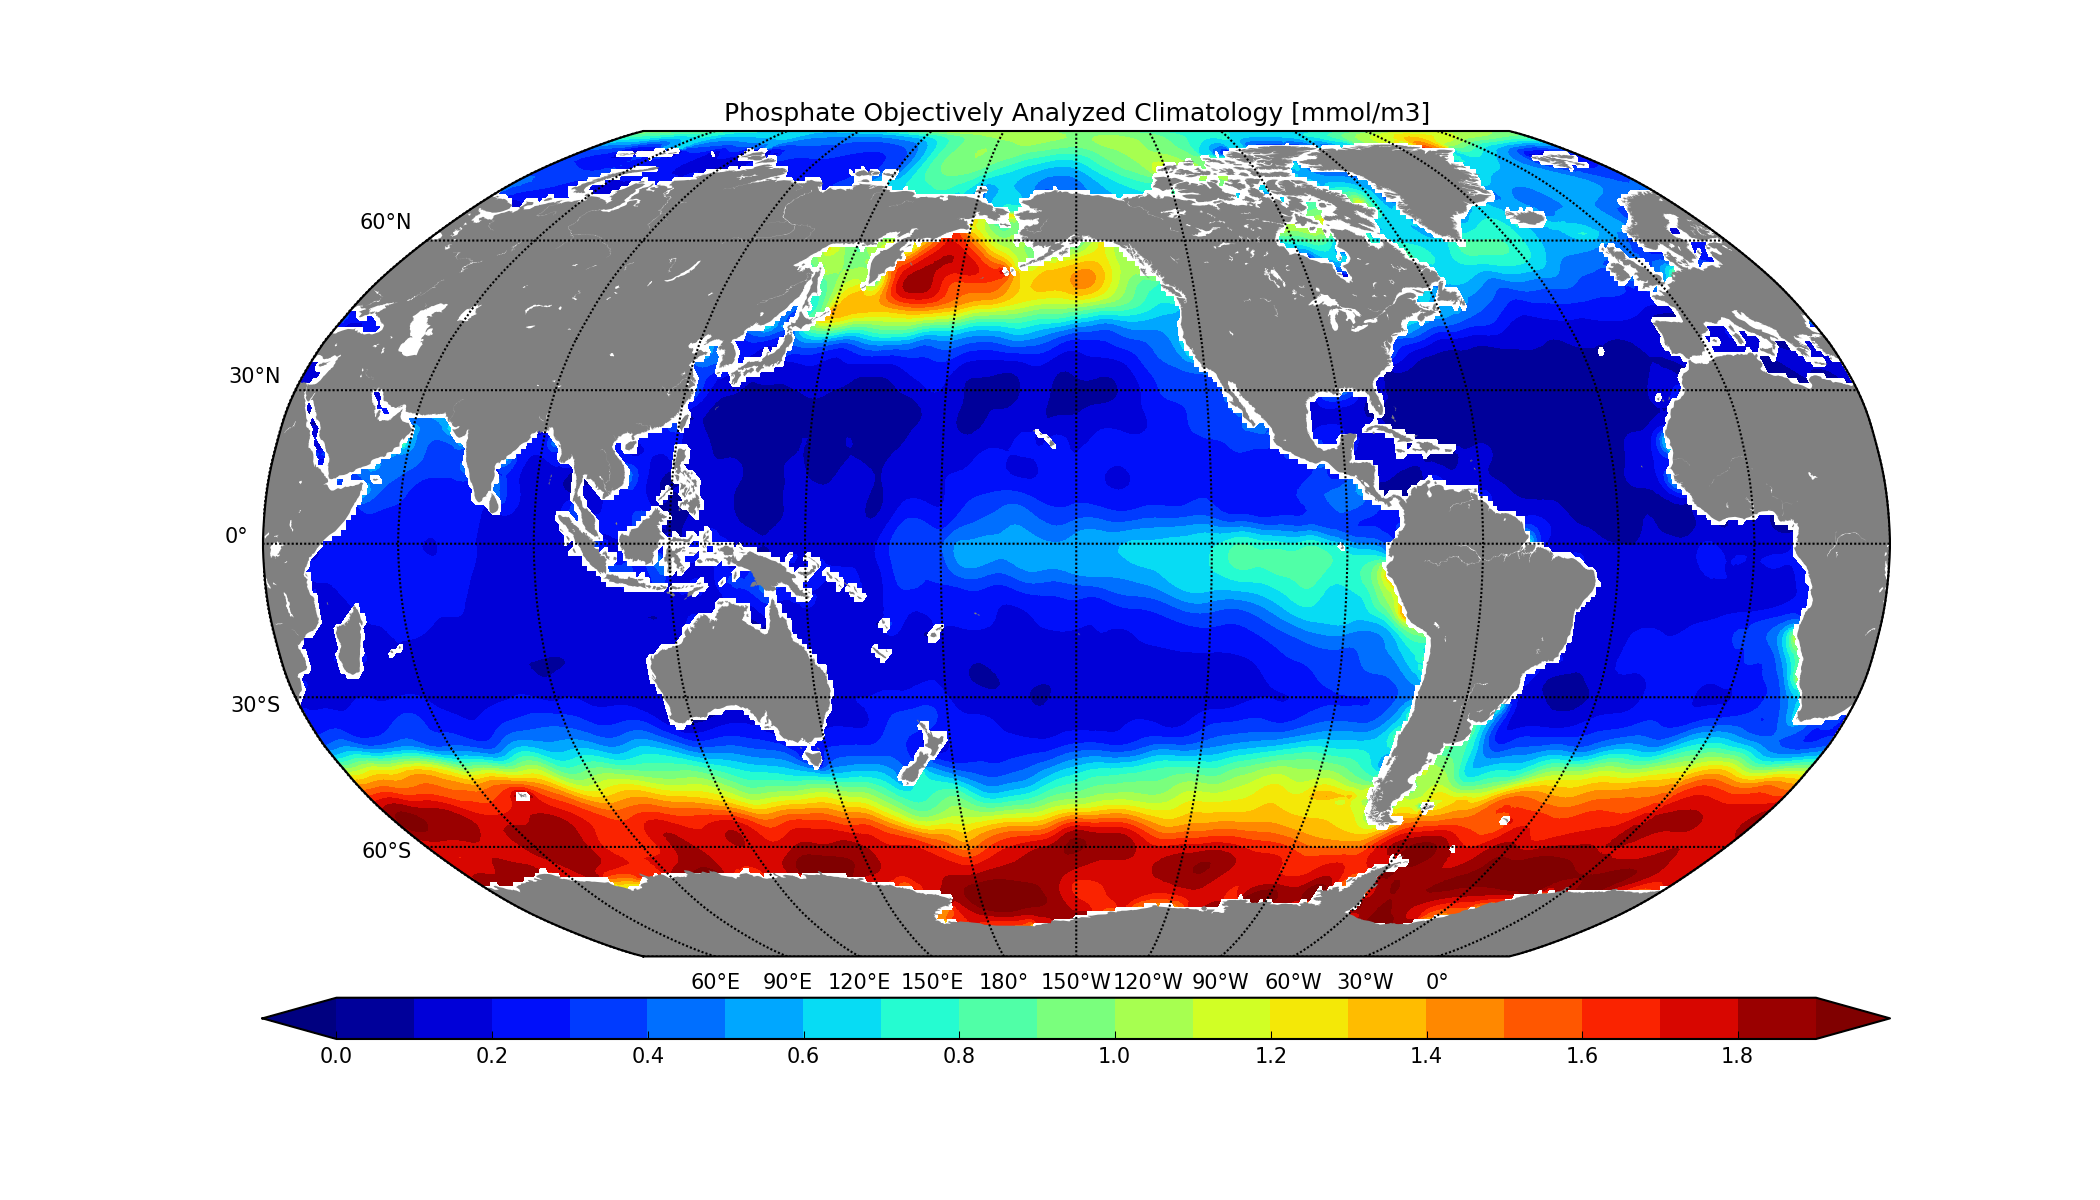
\includegraphics[width=7cm]{figures/M1/Phosphate_map_WOA9_python}

\column{5cm}
\begin{itemize}
\item Surface mean annual concentrations of oxygen and phosphate from the
World Ocean Atlas (WOA13) gridded dataset (1 deg x 1 deg)
\item This is a contour filled plot. The colormap is discrete, and it is
possible to appreciate the values.
\end{itemize}
\end{columns}

\end{frame}

\begin{frame}{Examples of scalar fields (sections)}

\begin{columns}[t]


\column{9cm}

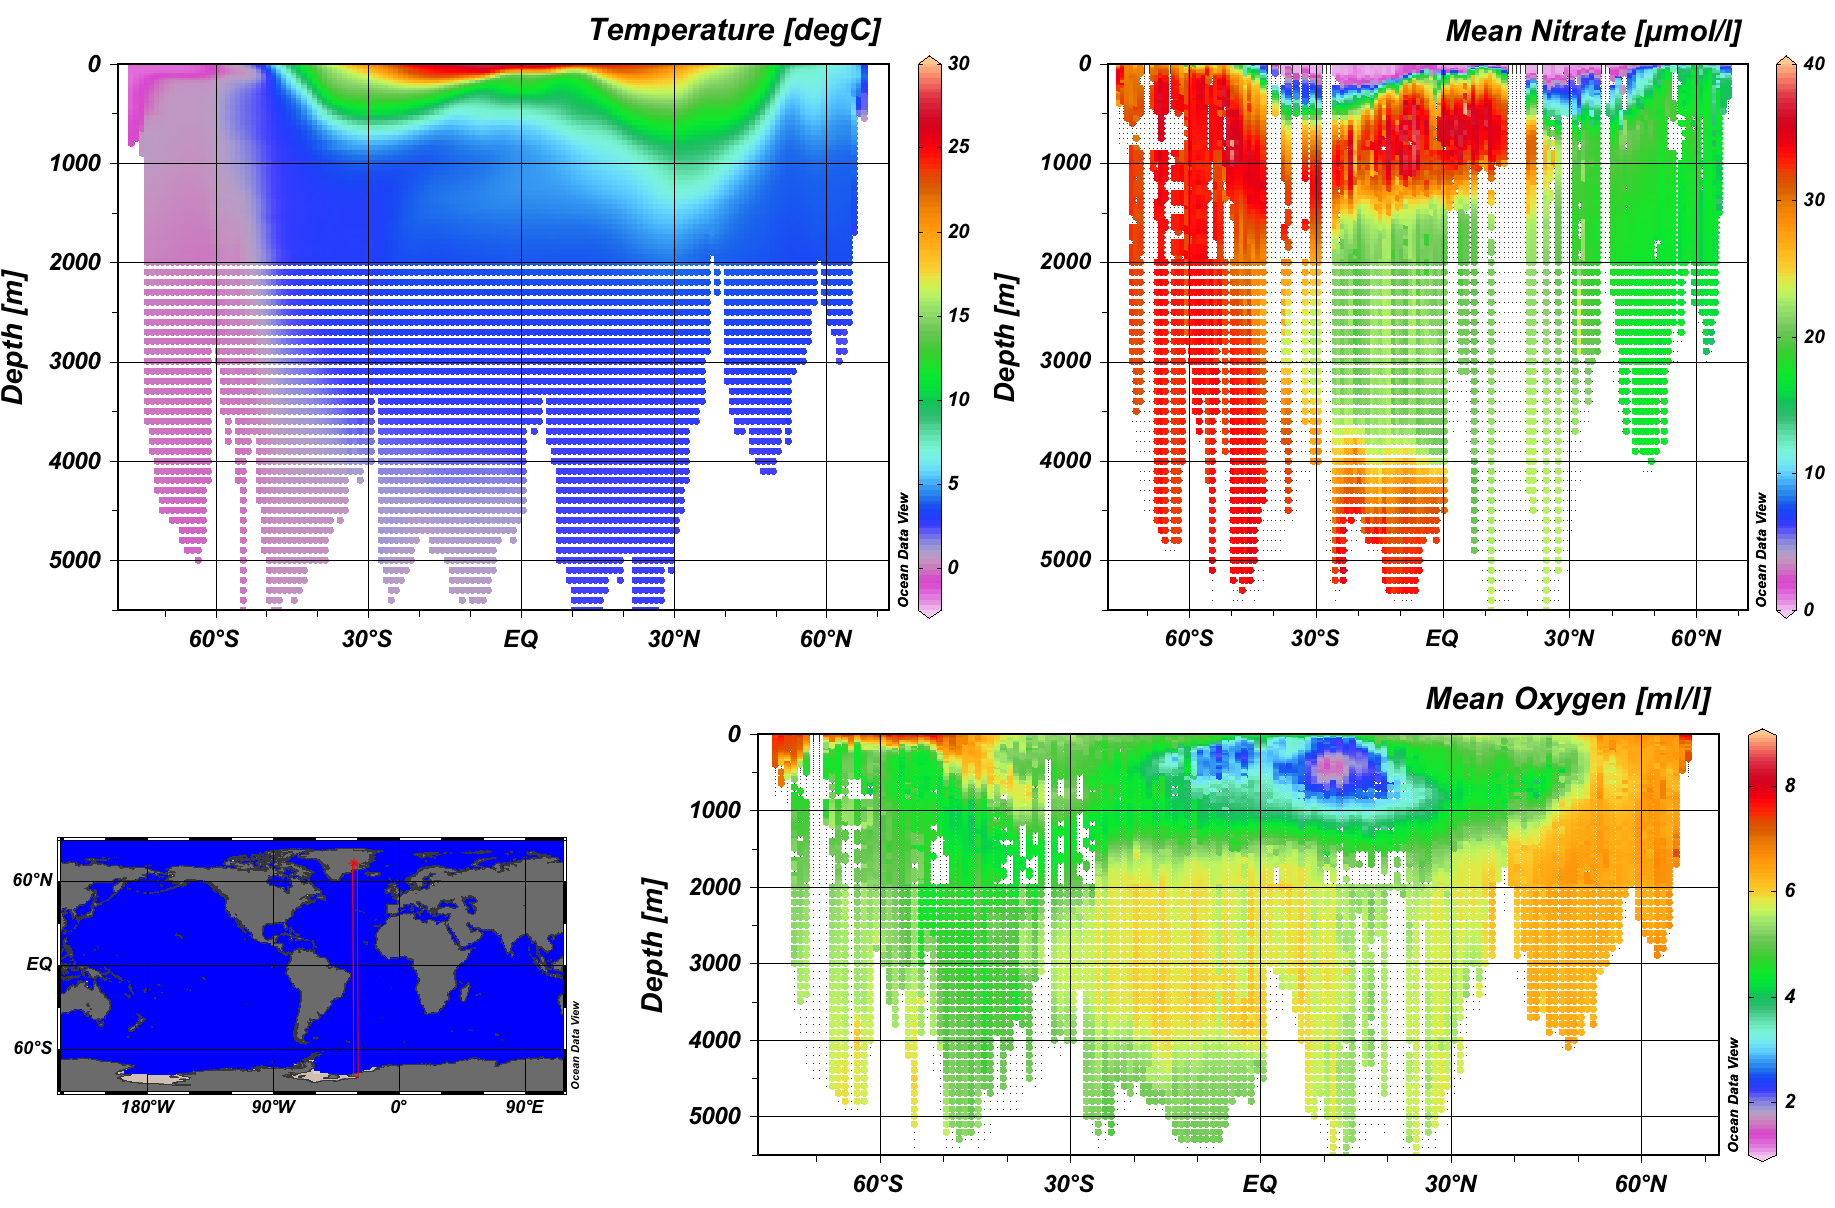
\includegraphics[width=9cm]{figures/M1/Sections_WOA13_ODV}

\column{3.5cm}
\begin{itemize}
\item Temperature, Nitrate and oxygen concentration in the Atlantic from
the World Ocean Atlas (WOA13) gridded dataset
\end{itemize}
\end{columns}

\end{frame}


\section{Vector fields}
\begin{frame}{Vectors in ocean and atmosphere science}

\begin{itemize}
\item The typical vector fields are wind or current velocities. They are
expressed in terms of components along the 3 spatial dimensions: $\vec{U}=\mathbf{U}=\left(u,v,w\right)$.
\uline{Each component is a scalar field} 
\item Operations on vectors and scalars can be done with the following \textbf{space
operators}:

\begin{itemize}
\item \textbf{the gradient} (the pressure gradient): computed on scalar
fields, produces vector fields 
\item \textbf{the divergence }(the fluid divergence): applied to vector
fields, produces a scalar field
\item \textbf{the curl }(the wind stress curl): computed on vector fields,
produces vector fields
\end{itemize}
\end{itemize}
\end{frame}

\begin{frame}{Examples of mathematical vector fields}

\begin{columns}[t]


\column{8cm}

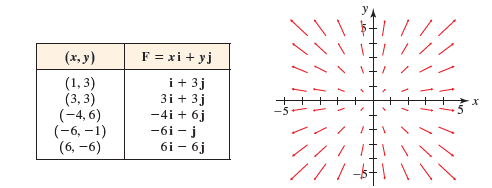
\includegraphics[width=10cm]{figures/M3/example_vector_field}

\column{4cm}
\begin{itemize}
\item A vector field is a function that \textbf{assigns a vector} to each
point on the coordinate plane
\item For every pair of coordinates, the function gives the components of
the vector
\[
\boldsymbol{F}\left(x,y\right)=x\boldsymbol{i}+y\boldsymbol{j}
\]
\end{itemize}
\end{columns}

\end{frame}

\begin{frame}{Atmospheric fields: wind stress}

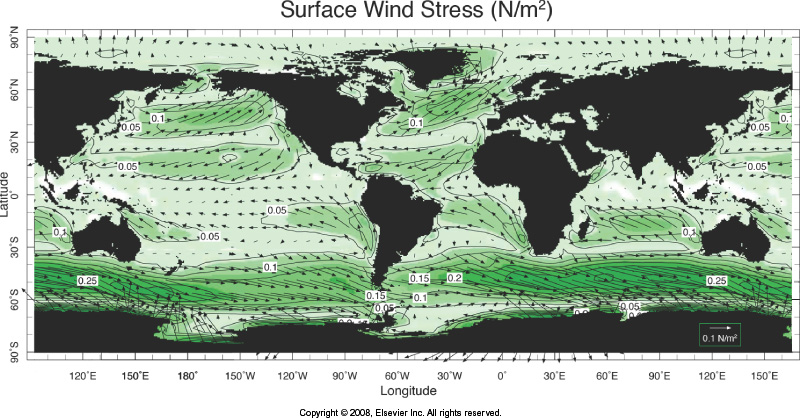
\includegraphics[scale=0.4]{figures/M1/MP_10_02_wstress.jpg}

{\footnotesize{}This field is derived from observations that have
been blended with a numerical model to obtain a regular grid. Wind
stress intensity (scalar) and wind vectors (Marshall and Plumb, Fig.
10.2)}{\footnotesize\par}
\end{frame}

\section{Operations on Scalar and Vector fields}

\begin{frame}{Scalar and vector operators}

\begin{itemize}
\item It is possible and useful to describe any scalar and vector field
(sea surface temperature in the South Atlantic or the Benguela velocity
field) by means of certain operators that provide quantitative indications
of their features
\item This is simpler to understand in the case of a mountain topography
or bathymetry along the coast: how do we know the steepness of the
mountain we are going to climb?
\item In the case of vector fields we will find out that some major relationships
between wind and currents can be obtained by rearranging the dynamical
equations using \textbf{vector operators}
\item A fully guided introduction to multi-variate scalar and vector functions
is available at the Khan Academy \url{https://www.khanacademy.org/math/multivariable-calculus/multivariable-derivatives}
\end{itemize}
\end{frame}

\begin{frame}{Warning: Matrix and Cartesian coordinates}

\begin{fact}
The natural direction of matrix and Cartesian coordinates is opposite!
A matrix is given as rows and columns, with the first index going
from the upper row downward and the second index from the first column
to the right (\emph{IJ-system}). In Cartesian coordinates (and geographic
graticule) the origin is in the lower left corner and the y-axis is
oriented upward (\emph{XY-system}).
\end{fact}

\begin{itemize}
\item It is important to keep this in mind when doing operations on matrices
that represent physical oceanographic or atmospheric fields
\item This is why a physical field is always given with the corresponding
coordinate matrices so that it is uniquely determined on the map.
Sea-level pressure $P_{sl}(x,y,t)$ should always have an indication
of the grid coordinates or two additional geographic grid fields:
$\phi(x,y)$ for latitude and $\lambda(x,y)$ for longitude.
\end{itemize}
\end{frame}

\begin{frame}{Fields and coordinate systems}

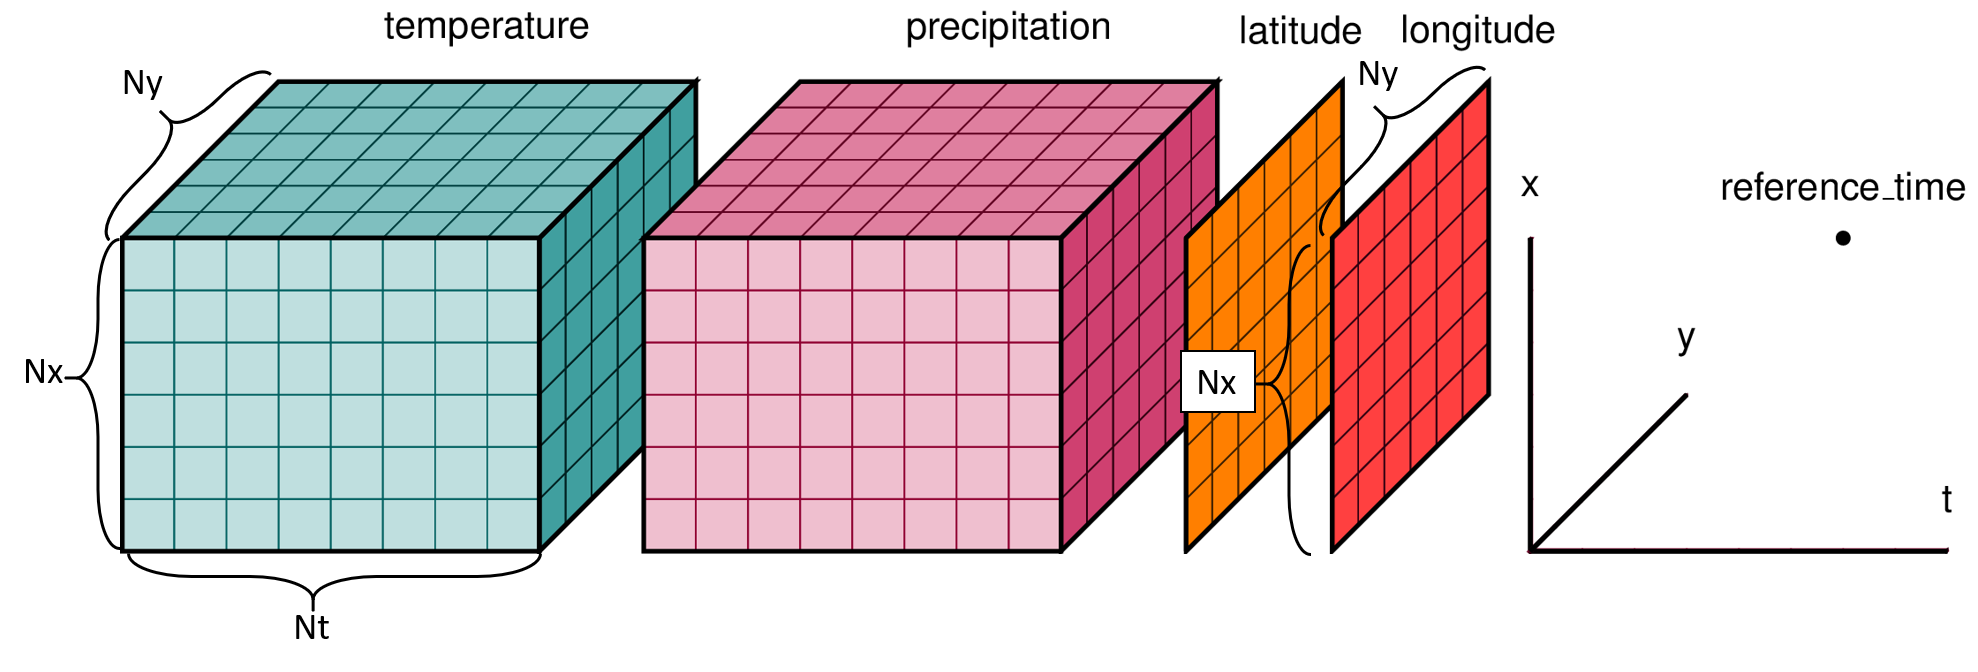
\includegraphics[scale=0.3]{figures/M3/dataset-diagram}

{\footnotesize{}Geoscientific fields are matrices that are referenced
to a system of coordinate. In the example above, sea surface temperature
and precipitation are represented as 3-D fields, with a number of
grid points along the x and y directions and a number of records along
the time axis (the indices of the matrix, $N_{x}\times N_{y}\times N_{t}$
in total. They are associated to two scalar fields containing the
corresponding latitude and longitude on the Earth (for every pair
of indices on the x-y plane). In summary, we have different objects:
}\textbf{\footnotesize{}indices, coordinates and variables}{\footnotesize{} }{\footnotesize\par}
\end{frame}


\section{The gradient of a field}
\begin{frame}{The gradient of a scalar field}

\begin{columns}[t]


\column{6cm}
\begin{itemize}
\item {\footnotesize{}This is the mean Sea level Pressure field for December
2014 taken from a typical meteorological data product called }\emph{\footnotesize{}atmospheric
reanalyses}{\footnotesize{} \url{http://www.esrl.noaa.gov/psd/data/gridded/data.ncep.reanalysis.surface.html}}{\footnotesize\par}
\item {\footnotesize{}It shows the subtropical highs and subpolar lows,
and the use of isolines allows to better see the changes}{\footnotesize\par}
\item {\footnotesize{}Pressure differences drive the wind and we know more
about the field if we compute the }\textbf{\footnotesize{}gradients}{\footnotesize\par}
\end{itemize}

\column{6cm}

\begin{figure}[t!]\vspace{-1cm}

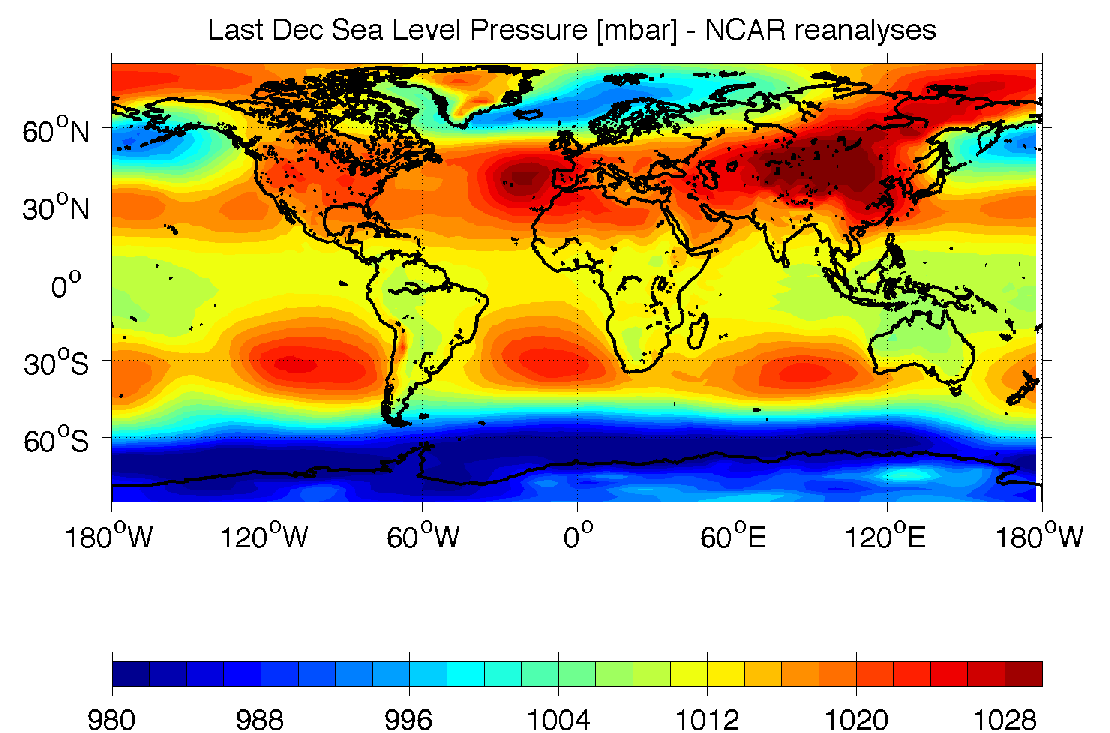
\includegraphics[width=5cm]{figures/M3/NCAR_slp_lastdec}\\
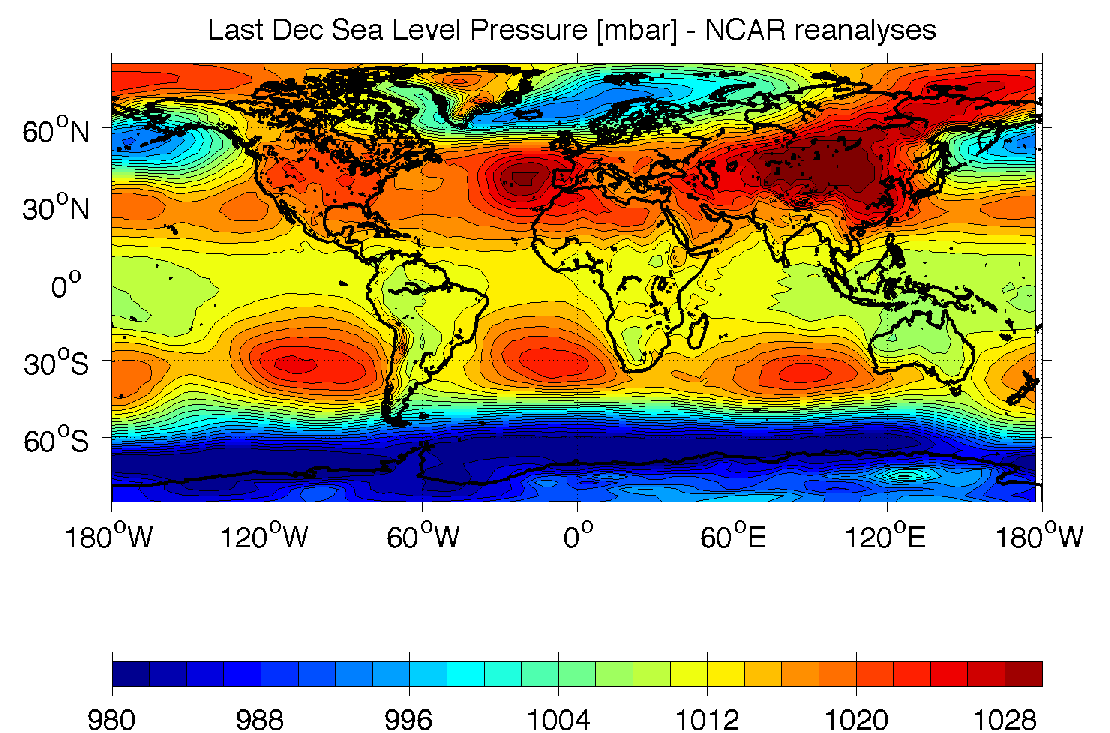
\includegraphics[width=5cm]{figures/M3/NCAR_slp_lastdec_line}

\end{figure}
\end{columns}

\end{frame}

\begin{frame}{The pressure gradient vector}

\begin{columns}[t]


\column{8cm}
\begin{itemize}
\item {\footnotesize{}The gradient is a vector because it measures the difference
in the scalar value across each dimension}{\footnotesize\par}
\item {\footnotesize{}On the geographical grid we talk about }\textbf{\footnotesize{}meridional}{\footnotesize{}
(north-south) and }\textbf{\footnotesize{}zonal}{\footnotesize{} (east-west)
gradient, therefore we have 2 components}{\footnotesize\par}
\item {\footnotesize{}The gradient of SLP is higher where pressure changes
the most per unit of space. The largest gradient is found in the meridional
component}{\footnotesize\par}
\end{itemize}
\begin{fact}
Gradients are positive or negative depending on the orientation of
the coordinate system 
\end{fact}


\column{6cm}

\begin{figure}[t!]\vspace{-1cm}

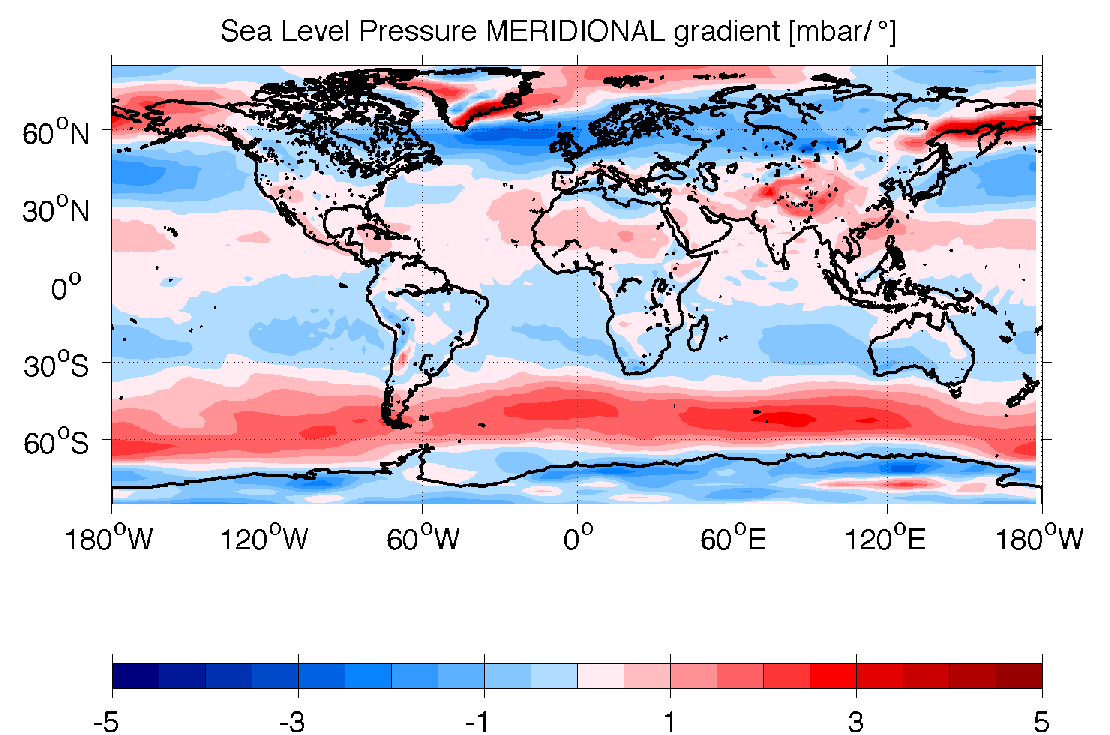
\includegraphics[width=5cm]{figures/M3/NCAR_slp_Ygrad_lastdec}\\
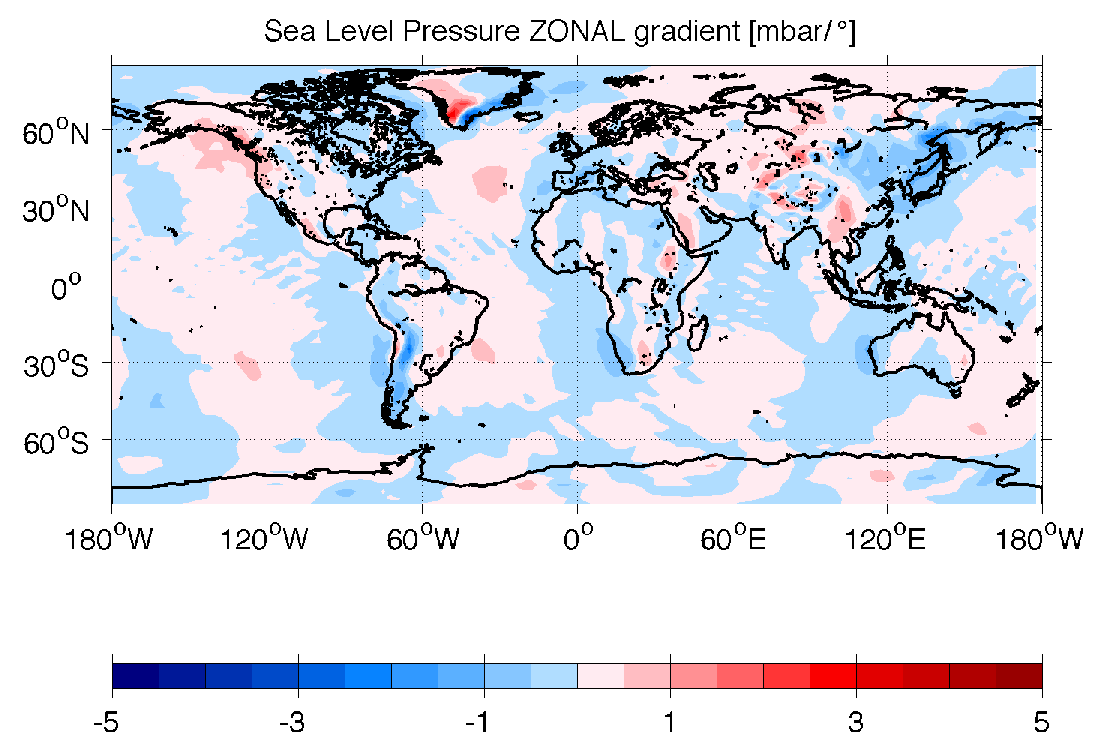
\includegraphics[width=5cm]{figures/M3/NCAR_slp_Xgrad_lastdec}\end{figure}
\end{columns}

\end{frame}

\begin{frame}{The ``nabla'' or ``del'' operator }

\begin{itemize}
\item The gradient of a 3-D field $P\left(x,y,z\right)$ is mathematically
described by the vector
\[
\boldsymbol{\psi}=\vec{\psi=}\left(\frac{\partial P}{\partial x},\frac{\partial P}{\partial y},\frac{\partial P}{\partial z}\right)=\frac{\partial P}{\partial x}\mathbf{\hat{i}}+\frac{\partial P}{\partial y}\mathbf{\hat{j}}+\frac{\partial P}{\partial z}\mathbf{\hat{k}}
\]
\item This is seen as the application of the operator \emph{nabla} or \emph{del}
\[
\nabla\equiv\left(\frac{\partial}{\partial x},\frac{\partial}{\partial y},\frac{\partial}{\partial z}\right)
\]
 to the field
\item Nabla is a vector and we formally multiply a vector by a scalar to
obtain the gradient vector
\[
\boldsymbol{\psi}=\boldsymbol{\nabla}P
\]
\end{itemize}
\end{frame}

\begin{frame}{The gradient of a vector field}

\begin{itemize}
\item A vector field is a collection of scalar fields, each one representing
the component of the vector along each direction
\item Considering the wind vector field $\mathbf{U}=\left(u,v,w\right)$,
we can apply the gradient to each scalar component
\item The gradient of the wind vector field is thus a matrix , where each
row represents the gradient applied to every component
\[
\nabla\mathbf{U}=\begin{bmatrix}\frac{\partial u}{\partial x} & \frac{\partial u}{\partial y} & \frac{\partial u}{\partial z}\\
\frac{\partial v}{\partial x} & \frac{\partial v}{\partial y} & \frac{\partial v}{\partial z}\\
\frac{\partial w}{\partial x} & \frac{\partial w}{\partial y} & \frac{\partial w}{\partial z}
\end{bmatrix}
\]
 
\end{itemize}
\end{frame}

\begin{frame}{The nabla operator with vector fields}

\begin{itemize}
\item When the operator vector nabla $\vec{\nabla}$ is \textbf{applied
to a vector}, we can obtain either a scalar or another vector depending
on the operation
\begin{itemize}
\item The \emph{dot product} gives a quantity called the \textbf{divergence}
of the vector field, which is a \textbf{scalar
\[
\boldsymbol{\nabla}\cdot\boldsymbol{V}
\]
}
\item The \emph{cross product} gives a quantity called the \textbf{curl}
of the vector field, which is a \textbf{vector
\[
\boldsymbol{\nabla}\times\boldsymbol{V}
\]
}
\end{itemize}
\end{itemize}
\end{frame}


\section{The divergence of a vector field}
\begin{frame}{Divergence}

\begin{itemize}
\item Divergence is the mathematical expression of the principle of mass
conservation or continuity (more in Module 3)
\item If the vector field is fluid velocity (current or wind, $\boldsymbol{U}\equiv\left(u,v,w\right)$)
then the divergence of the field measures the local change of flow
through an infinitesimally small volume
\[
\boldsymbol{\nabla}\cdot\boldsymbol{U}=\left(\frac{\partial}{\partial x},\frac{\partial}{\partial y},\frac{\partial}{\partial z}\right)\cdot\left(u,v,w\right)=\frac{\partial u}{\partial x}+\frac{\partial v}{\partial y}+\frac{\partial w}{\partial z}
\]
\item If we are interested in the amount of water or air or the concentration
of a nutrient, then the principle is better written as the divergence
of the density (or concentration) flux 
\[
\boldsymbol{\nabla}\cdot\left(\rho\boldsymbol{U}\right)=-\frac{\partial\rho}{\partial t}
\]
\end{itemize}
\end{frame}

\begin{frame}{Visual interpretation of the divergence}

\begin{itemize}
\item Which of these fields have divergence different from 0?
\item The 1st and 3rd fields show divergent and convergent flows. These
fields will have a divergence that is non-zero. For all the other
fields, you can draw any closed line and you will always have an equal
flow through the line
\end{itemize}
\begin{center}
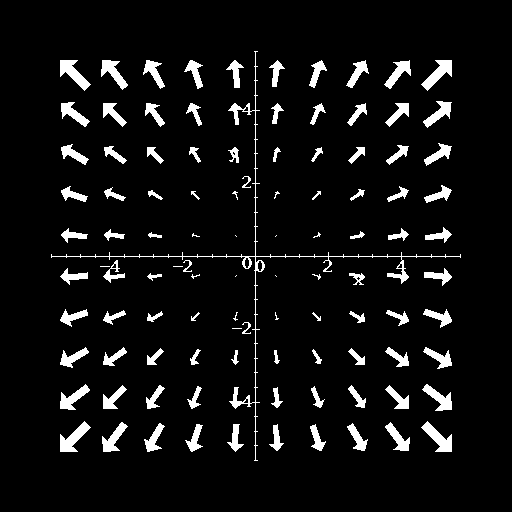
\includegraphics[scale=0.15]{figures/M3/div_field1}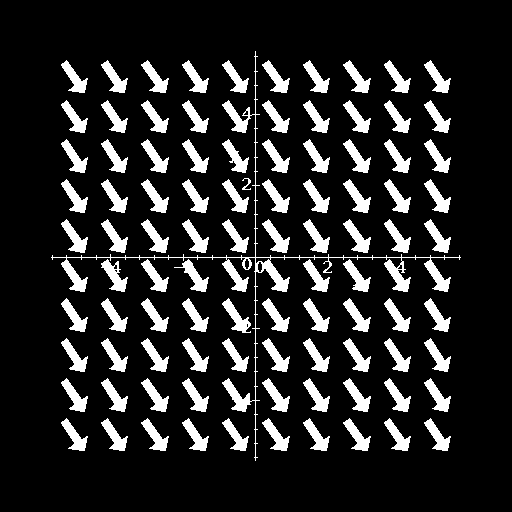
\includegraphics[scale=0.15]{figures/M3/div_field2}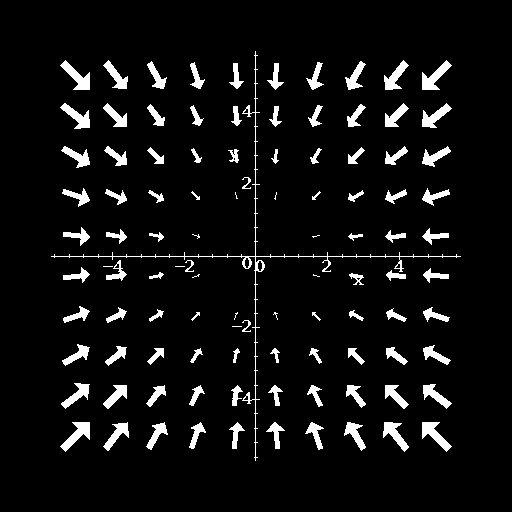
\includegraphics[scale=0.15]{figures/M3/div_field3}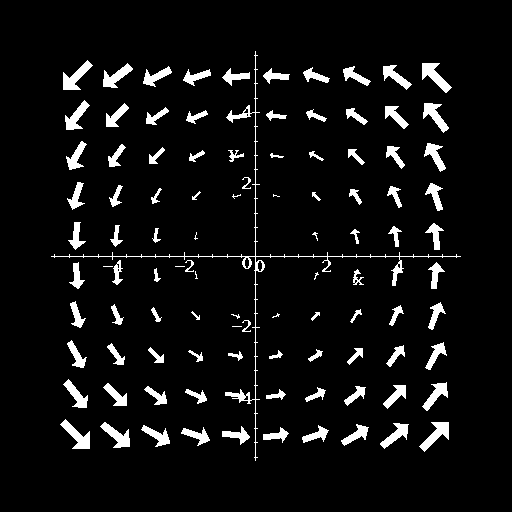
\includegraphics[scale=0.15]{figures/M3/div_field4}
\par\end{center}

\url{http://citadel.sjfc.edu/faculty/kgreen/vector/block2/del_op/node5.html}
\end{frame}


\section{The curl of a vector field}
\begin{frame}{Curl}

\begin{itemize}
\item Curl is the mathematical expression of the amount of \textquotedbl rotation\textquotedbl{}
or angular momentum of the fluid. 
\item If the vector field is fluid velocity (current or wind, $\boldsymbol{U}\equiv\left(u,v,w\right)$)
then the curl of the field measures the rotation of flow around an
infinitesimally small closed line over a plane. We apply the rule
of the cross or vector product seen in M1W1. 
\[
\boldsymbol{\nabla}\times\boldsymbol{U}=\begin{vmatrix}\mathbf{\hat{i}} & \mathbf{\hat{j}} & \mathbf{\hat{k}}\\
\partial_{x} & \partial_{y} & \partial_{z}\\
u & v & w
\end{vmatrix}=\left(\frac{\partial w}{\partial y}-\frac{\partial v}{\partial z}\right)\mathbf{\hat{i}}-\left(\frac{\partial w}{\partial x}-\frac{\partial u}{\partial z}\right)\mathbf{\hat{j}}+\left(\frac{\partial v}{\partial x}-\frac{\partial u}{\partial y}\right)\mathbf{\hat{k}}
\]
\item It is a vector because it also gives information on the \textbf{orientation
of the plane} over which the circulation occurs: the curl is by definition
\textbf{perpendicular} to that plane 
\end{itemize}
\end{frame}

\begin{frame}{Visual interpretation of the curl}

\begin{itemize}
\item Which of these fields have curl different from 0?
\item The only clear rotational field is the last one. The 1st and 3d field
could also have a rotational component 
\end{itemize}
\begin{center}
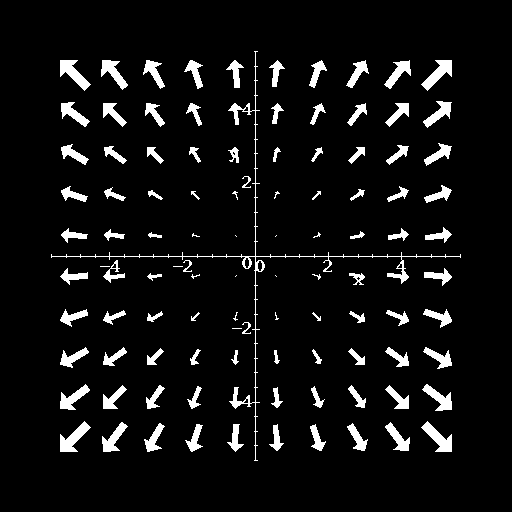
\includegraphics[scale=0.15]{figures/M3/div_field1}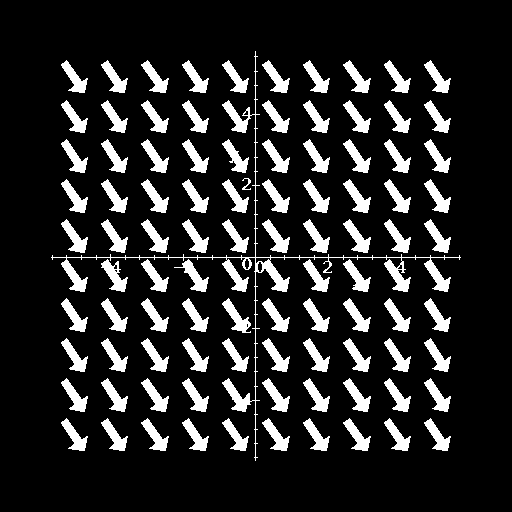
\includegraphics[scale=0.15]{figures/M3/div_field2}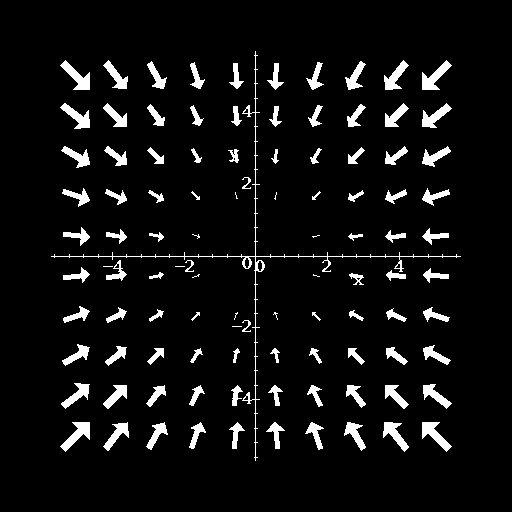
\includegraphics[scale=0.15]{figures/M3/div_field3}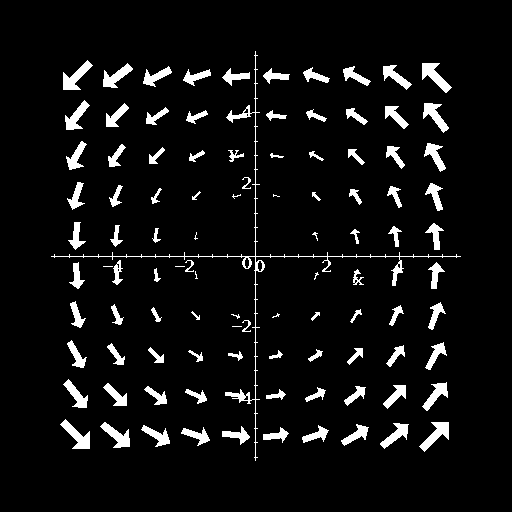
\includegraphics[scale=0.15]{figures/M3/div_field4}
\par\end{center}

\url{http://citadel.sjfc.edu/faculty/kgreen/vector/block2/del_op/node9.html}
\end{frame}

\begin{frame}{Useful properties}

\begin{itemize}
\item The advantage of the gradient and curl operators will become clear
when deriving the equations for geophysical fluid dynamics
\item The following properties will be very useful in the future (try to
demonstrate them using the components)

\begin{itemize}
\item the curl of the gradient of a scalar field is null: $\nabla\times\left(\nabla\phi\right)=0$
\item the divergence of the curl of a vector field is null: $\nabla\cdot\left(\nabla\times\mathbf{u}\right)=0$
\end{itemize}
\end{itemize}
\end{frame}


\end{document}
